\chapter{绪论}

% \begin{figure}[h]
%     \centering
%     
\includegraphics[width=0.5\textwidth]{figures/R-C.jpg}
%     \caption{常见的牛马形象}
%     \end{figure}
    
% \section{研究背景与意义}
% 主要组织相容性复合体（Major Histocompatibility Complex，MHC）分子在适应性免疫应答过程中起着关键作用。其中，MHC-I 分子能够将细胞内来源的肽段递呈至细胞表面，并被 CD8+ T 细胞识别，从而触发后续免疫反应\cite{koh2023cd8}。因此，MHC-I 与肽段的结合能力是抗原递呈过程中的核心环节，围绕 MHC-I 结合肽反应展开预测，也逐渐成为肿瘤新抗原筛选、疫苗设计、免疫治疗和免疫多肽组学等领域的重要研究内容\cite{xie2023neoantigens}。

% 近年来，高通量测序、质谱技术和蛋白质组学研究发展很快，相关的 HLA 及其结合肽数据不断积累，为基于计算方法开展 MHC-I 结合肽预测提供了较好的数据基础\cite{vita2025iedb,thibault2022immunopeptidomics}。与此同时，深度学习在生物信息学中的应用不断拓展，使序列表征能力得到明显提升。相比依赖基序、打分矩阵或浅层机器学习的方法，深度学习模型能够更充分地挖掘 HLA 序列和候选肽段序列中的复杂特征，因此在预测性能和泛化能力上表现出更大优势\cite{lin2023evolutionary,xu2024immuneapp}。

% 将重操作后
适应性免疫应答离不开主要组织相容性复合体（Major Histocompatibility Complex，MHC）分子所发挥的核心功能。其中，MHC-I 分子负责将内源性肽段递呈至细胞表面，供 CD8 T 细胞识别，进而启动下游免疫反应\cite{koh2023cd8}。可见，肽段与 MHC-I 的结合能力是抗原递呈过程中的决定性环节，针对 MHC-I 结合肽的预测研究亦由此在肿瘤新抗原筛选、疫苗设计、免疫治疗与免疫多肽组学等领域占据重要位置\cite{xie2023neoantigens}。

高通量测序、质谱及蛋白质组学技术的快速进步，使得 HLA（同 MHC-I，为同一分子） 及其结合肽数据规模持续扩大，这为基于计算策略的 MHC-I 结合肽预测工作提供了更充实的数据基础\cite{vita2025iedb,thibault2022immunopeptidomics}。同时，深度学习在生物信息学中的渗透程度不断提高，序列表征能力也因此显著增强。相较于依赖基序、打分矩阵或浅层机器学习的原有方法，深度学习模型能够更深入地捕获 HLA 序列与候选肽段序列中的复杂模式，因而在预测准确度与泛化性能上表现出更明显的优势\cite{lin2023evolutionary,xu2024immuneapp}。

在这一背景下，FennOmix.MHC 作为面向 MHC-I 肽段结合预测的深度学习模型，将 HLA/MHC-I 蛋白序列和候选肽段序列作为两个模态输入，通过对比学习将真实结合对在共享嵌入空间中拉近，并将随机负样本推远，从而实现基于距离关系的结合预测与候选筛选。该模型不仅能够完成 MHC-I 肽段结合预测，还具备支持候选肽段检索、缩库辅助搜库等下游任务的潜力，因此具有一定的应用基础。

% 然而，当 FennOmix.MHC 进一步应用到大规模人类蛋白质组场景时，工程部署问题逐渐突出。在典型应用中，需要将人类常见蛋白质序列切分为不同长度的候选肽段，候选规模可达到数千万级。若继续采用原始高维 float32 向量表示，预编码肽段缓存将占用大量存储空间，不仅难以完整放入单块 GPU 显存或普通主机内存中，也会增加磁盘占用、I/O 访问、多进程传输、部署备份和版本管理等方面的压力，最终影响模型在实际环境中的使用效率。

% 将重操作后
然而，将 FennOmix.MHC 推向大规模人类蛋白质组分析时，其工程化部署面临的挑战日益凸显。在典型分析流程中，需先将人类常见蛋白质序列切割成不同长度的候选肽段，候选规模常可达数千万条。若沿用原始的高维 float32 向量表示，预编码肽段缓存将消耗庞大的存储开销：不仅难以整体容纳于单块 GPU 显存或普通主机内存，还会显著加重磁盘占用、I/O 访问、多进程传输、部署备份及版本管理等环节的负担，进而严重制约模型在真实部署环境中的使用效率。

% 从系统角度看，这一问题并不只是“模型参数多”或“单次推理慢”所导致，而是由表示维度、缓存方式、检索流程和运行环境共同形成的综合瓶颈。高维向量会直接增加离线缓存和在线检索成本，频繁的数据加载和跨进程传输又会进一步放大 I/O 压力。同时，模型结构中也可能存在一定冗余，推理过程仍有继续压缩和优化的空间。因此，围绕 FennOmix.MHC 开展轻量化和部署优化，不仅具有明确的工程价值，也具有一定的方法研究意义。

% 与单纯提出新的预测模型不同，本文更关注已有深度学习模型在大规模候选肽段场景中的工程可用性，重点分析模型表示、缓存管理和在线检索之间的协同优化问题。本文围绕 FennOmix.MHC 在大规模人类蛋白质组场景中的部署需求，关注高维缓存、存储开销、I/O 压力和推理冗余等问题，探索兼顾预测性能与工程可用性的优化方案。本文研究意义主要体现在以下三个方面。

% 第一，在理论层面，本文尝试从“表示能力—存储成本—推理效率”的角度分析免疫多肽结合预测模型的部署瓶颈。现有研究通常更关注预测精度，而对模型在大规模候选库场景中的资源消耗讨论相对较少。将轻量化目标纳入模型设计和实验评估，有助于为该类模型的工程化研究提供新的分析视角\cite{li2023model}。

% 第二，在方法层面，本文将模型降维、结构剪枝、缓存量化和索引检索等方法结合起来，尝试形成一套面向部署场景的系统优化思路。该思路并不是单独优化某一个模型指标，而是从模型表示、结构冗余、缓存组织和查询执行多个层面共同降低系统开销，为深度学习模型在免疫多肽结合预测任务中的轻量化应用提供参考。

% 第三，在应用层面，本文研究可为大规模候选肽段筛选、缩库辅助搜库以及资源受限环境下的模型部署提供支持。特别是在真实质谱鉴定场景中，若能将模型预测与数据库检索结合起来，有望减少候选空间规模，降低后续搜库开销，从而增强模型的实际应用价值。

% 综合来看，针对 FennOmix.MHC 在大规模应用场景下面临的部署问题开展系统优化，既具有现实工程意义，也具有一定研究价值。

% 将重操作后
从系统层面审视，该瓶颈并非单纯源于模型参数量大或单次推理耗时，而是由表示维度、缓存策略、检索流程与运行环境共同塑造的复合约束。高维向量直接推高离线缓存与在线检索的开销，频繁的数据加载与跨进程传输则进一步加剧 I/O 负担；同时，模型内部也存在一定的结构冗余，推理链路仍有压缩与加速的余地。正因如此，围绕 FennOmix.MHC 开展轻量化与部署优化，既具备明确的工程价值，也蕴含方法层面的研究意义。

与提出全新预测架构的工作不同，本文更关注现有深度学习模型在大规模候选肽段场景下的工程可用性，重点关注模型表示、缓存管理和在线检索之间的协同优化。围绕 FennOmix.MHC 在人类蛋白质组规模下的部署需求，我们针对高维缓存、存储开销、I/O 压力和推理冗余等瓶颈，探索在保持预测能力的同时提升系统可用性的优化方案。其意义主要体现在三个方面。

在理论层面，本文从“表示能力—存储成本—推理效率”这三者的关系出发，重新审视免疫肽结合预测模型在部署中的瓶颈。目前多数工作仍聚焦于预测精度，对模型在大规模候选库下的资源消耗关注相对较少。将轻量化目标提前纳入模型设计和实验评估，有可能为该类模型的工程化研究提供一种不同于精度竞赛的分析视角\cite{li2023model}。

在方法层面，本文尝试融合模型降维、结构剪枝、缓存量化和索引检索等策略，形成一套面向部署的系统优化思路。这些手段并不追求某一指标的极致，而是从表示、结构、存储和查询四个环节同步降低开销，从而为深度学习免疫肽结合预测模型的轻量化落地提供方法参考。

在应用层面，所得方案可直接用于大规模候选肽段筛选、缩库辅助搜库以及资源受限环境下的模型部署。特别是在实际质谱鉴定流程中，如果将模型预测与数据库检索对接，就有可能先一步缩小候选空间，降低下游搜库的计算成本，明显增强模型在真实业务链路中的实用价值。

概括而言，针对 FennOmix.MHC 在大规模应用中所暴露的部署难题进行系统优化，不仅具有明确的工程落地意义，也具备一定的研究讨论价值。

\section{国内外研究现状}

\subsection{MHC-I 肽段结合预测研究进展}

MHC-I 与肽段的结合预测是免疫信息学的核心问题之一。早期方法主要依靠结合基序、位置特异性打分矩阵和浅层统计学习模型，通过肽段关键位置上的氨基酸偏好来推断与 MHC 分子的结合可能\cite{peters2005generating}。在数据量较小时，这类方法有一定实用性，但面对多样的等位基因、变化的肽长以及跨数据集泛化要求，其局限就变得相当突出。

进入机器学习与深度学习阶段后，该领域逐步从手工构造特征转向数据驱动的表示学习。当前较有代表性的模型包括 NetMHCpan\cite{reynisson2020netmhcpan}、MixMHCpred\cite{gfeller2023mixmhcpred}、ESM 系列\cite{rives2021biological} 和 FennOmix.MHC 等。文献调研显示，NetMHCpan 将短肽序列与 HLA 伪序列一并送入神经网络，并利用基序去卷积框架来改善对不同等位基因和肽长的适应能力；MixMHCpred 直接基于质谱鉴定的 HLA 结合肽，通过基序去卷积学习等位基因特异的位点概率矩阵和肽长分布；ESM 系列则借助海量蛋白质序列的预训练获得氨基酸的通用表示，为下游表位预测提供较高质量的嵌入特征。

与上述方法不同，FennOmix.MHC 采用了双模态编码和共享嵌入空间的设计，将 HLA/MHC-I 蛋白序列和候选肽段映射到同一表示空间，并通过深度对比学习拉近正样本对、推远负样本对。这一思路不仅适用于结合预测，也自然兼容候选肽段检索、数据库缩减和辅助搜库等任务，在功能延展性上具备一定优势。

整体来看，MHC-I 肽段结合预测已经形成了较为多元的方法体系，研究的重心也从单纯追求精度，逐步延伸到更强的表示能力、更好的跨等位基因泛化性以及更贴近真实应用场景的任务适配性\cite{reynisson2020netmhcpan,gfeller2023improved,abelin2024innovations}。不过，相比于模型性能的持续提升，围绕大规模候选肽库场景下的资源消耗和系统部署问题，现有的讨论还比较薄弱。

\subsection{深度学习模型轻量化与部署优化研究现状}

深度学习模型从实验环境走向实际部署，轻量化是不可回避的一步。模型规模持续膨胀所带来的参数量、存储成本、推理延迟和部署复杂度，已经成为制约应用落地的主要瓶颈。针对这些问题，降维、剪枝、量化、知识蒸馏等策略得到了广泛研究\cite{li2023model,cheng2024survey}。

在特征表示层面，降维是一种直接且有效的压缩方式。压缩嵌入向量的维度可以缩减缓存占用，并降低后续相似度计算与检索的时空开销。不同降维方法在压缩率、信息保真度和训练稳定性之间各有取舍：线性方案结构简单、参数量少，非线性方案则在保留复杂特征结构上具备理论优势\cite{sorzano2014survey,wang2016autoencoder}。

在模型结构层面，剪枝是去除冗余参数、减轻推理负担的常用手段。对于 Transformer 类模型，常见的剪枝目标包括注意力头和前馈网络的隐藏单元。通过评估各组件的重要性并裁剪贡献较低的部分，可以在不明显损害模型性能的前提下有效压缩结构复杂度\cite{michel2019sixteen,lagunas2021block}。

在缓存和部署层面，量化是压缩模型参数与向量存储体积的重要技术。将 float32 表示转换为 INT8 等低位宽格式，能显著缩减存储空间和数据搬运开销，但需要留意量化误差对后续检索和匹配环节的影响。另外，在大规模候选向量检索任务中，索引机制同样是部署优化不可忽视的一环。利用预计算缓存并配合哈希映射或向量索引结构，可以避免重复编码与无效遍历，从而提升在线查询的响应效率。

总体而言，轻量化与部署优化技术在通用深度学习领域已有较多探索，但以系统化的方式将它们引入免疫多肽结合预测模型的工作仍不多见，尤其是与大规模候选肽段缓存和下游缩库搜库等任务深度绑定的研究更为稀缺。这恰好为本文以 FennOmix.MHC 为对象，系统开展轻量化与部署优化留出了研究空间。

\subsection{现有工作存在的不足}
尽管 MHC-I 肽段结合预测方法在模型结构和预测精度上已取得长足进步，但从工程部署和应用落地的视角审视，仍存在若干短板。

其一，已有研究大多将提升预测精度作为首要目标，对模型在大规模实际场景中的资源消耗缺少系统性的剖析。面对数千万量级的候选肽段，高质量嵌入仅是必要条件，缓存体量、存储成本与加载效率同样决定着系统能否真正上线。

其二，模型优化与系统优化常被分开讨论。单纯压缩模型参数未必能解决高维缓存问题，单纯缩减缓存也未必能保住表示质量。因而，有必要将编码维度选择、模型结构压缩、缓存格式改造与检索流程设计统筹起来，形成面向部署的整体优化方案。

其三，现有轻量化研究大多缺少与真实下游任务打通的评价体系。对于免疫多肽结合预测模型，常规召回指标仅反映测试集上的表现，难以直接说明其在真实质谱搜库或大规模候选筛选中的实际价值。因此，有必要将轻量化方案与下游任务评价紧密挂钩，从预测效能、候选库保持能力和系统资源开销等多维视角综合判断方案的有效性。

基于以上不足，本文选取 FennOmix.MHC 作为具体研究对象，从表示压缩、结构轻量化、缓存压缩和索引检索等方面入手，尝试构建一套面向实际部署的系统优化方案。

\section{本文主要研究内容}

围绕 FennOmix.MHC 在大规模人类蛋白质组应用中遇到的高维缓存膨胀、推理开销偏高和部署困难等问题，本文从模型轻量化与系统工程优化两个方面展开，具体工作如下。

\begin{enumerate}[label=（\arabic*）, leftmargin=5em, itemsep=0pt, topsep=0pt]
    \item 搭建 FennOmix.MHC 基础实验环境，完成原模型复现。
    \item 探索模型输出维度的压缩方案，评估不同嵌入大小对性能与存储的影响。
    \item 对比线性和非线性降维策略，选取适合部署的默认设置。
    \item 分析模型结构冗余，寻找可行的剪枝路径。
    \item 设计面向肽段缓存的量化压缩方法，缓解存储和加载压力。
    \item 构建大规模肽段索引与在线查询流水线，提升筛选效率。
\end{enumerate}

通过以上工作，本研究试图为 FennOmix.MHC 构建一套面向实际部署的优化方案，在保持较高预测能力的同时，显著压缩存储与推理开销，进而增强其在大规模肽段筛选和下游搜库任务中的实用性。整体技术路线如图~\ref{fig:tech-route}所示。

\begin{figure}[htbp]
\centering
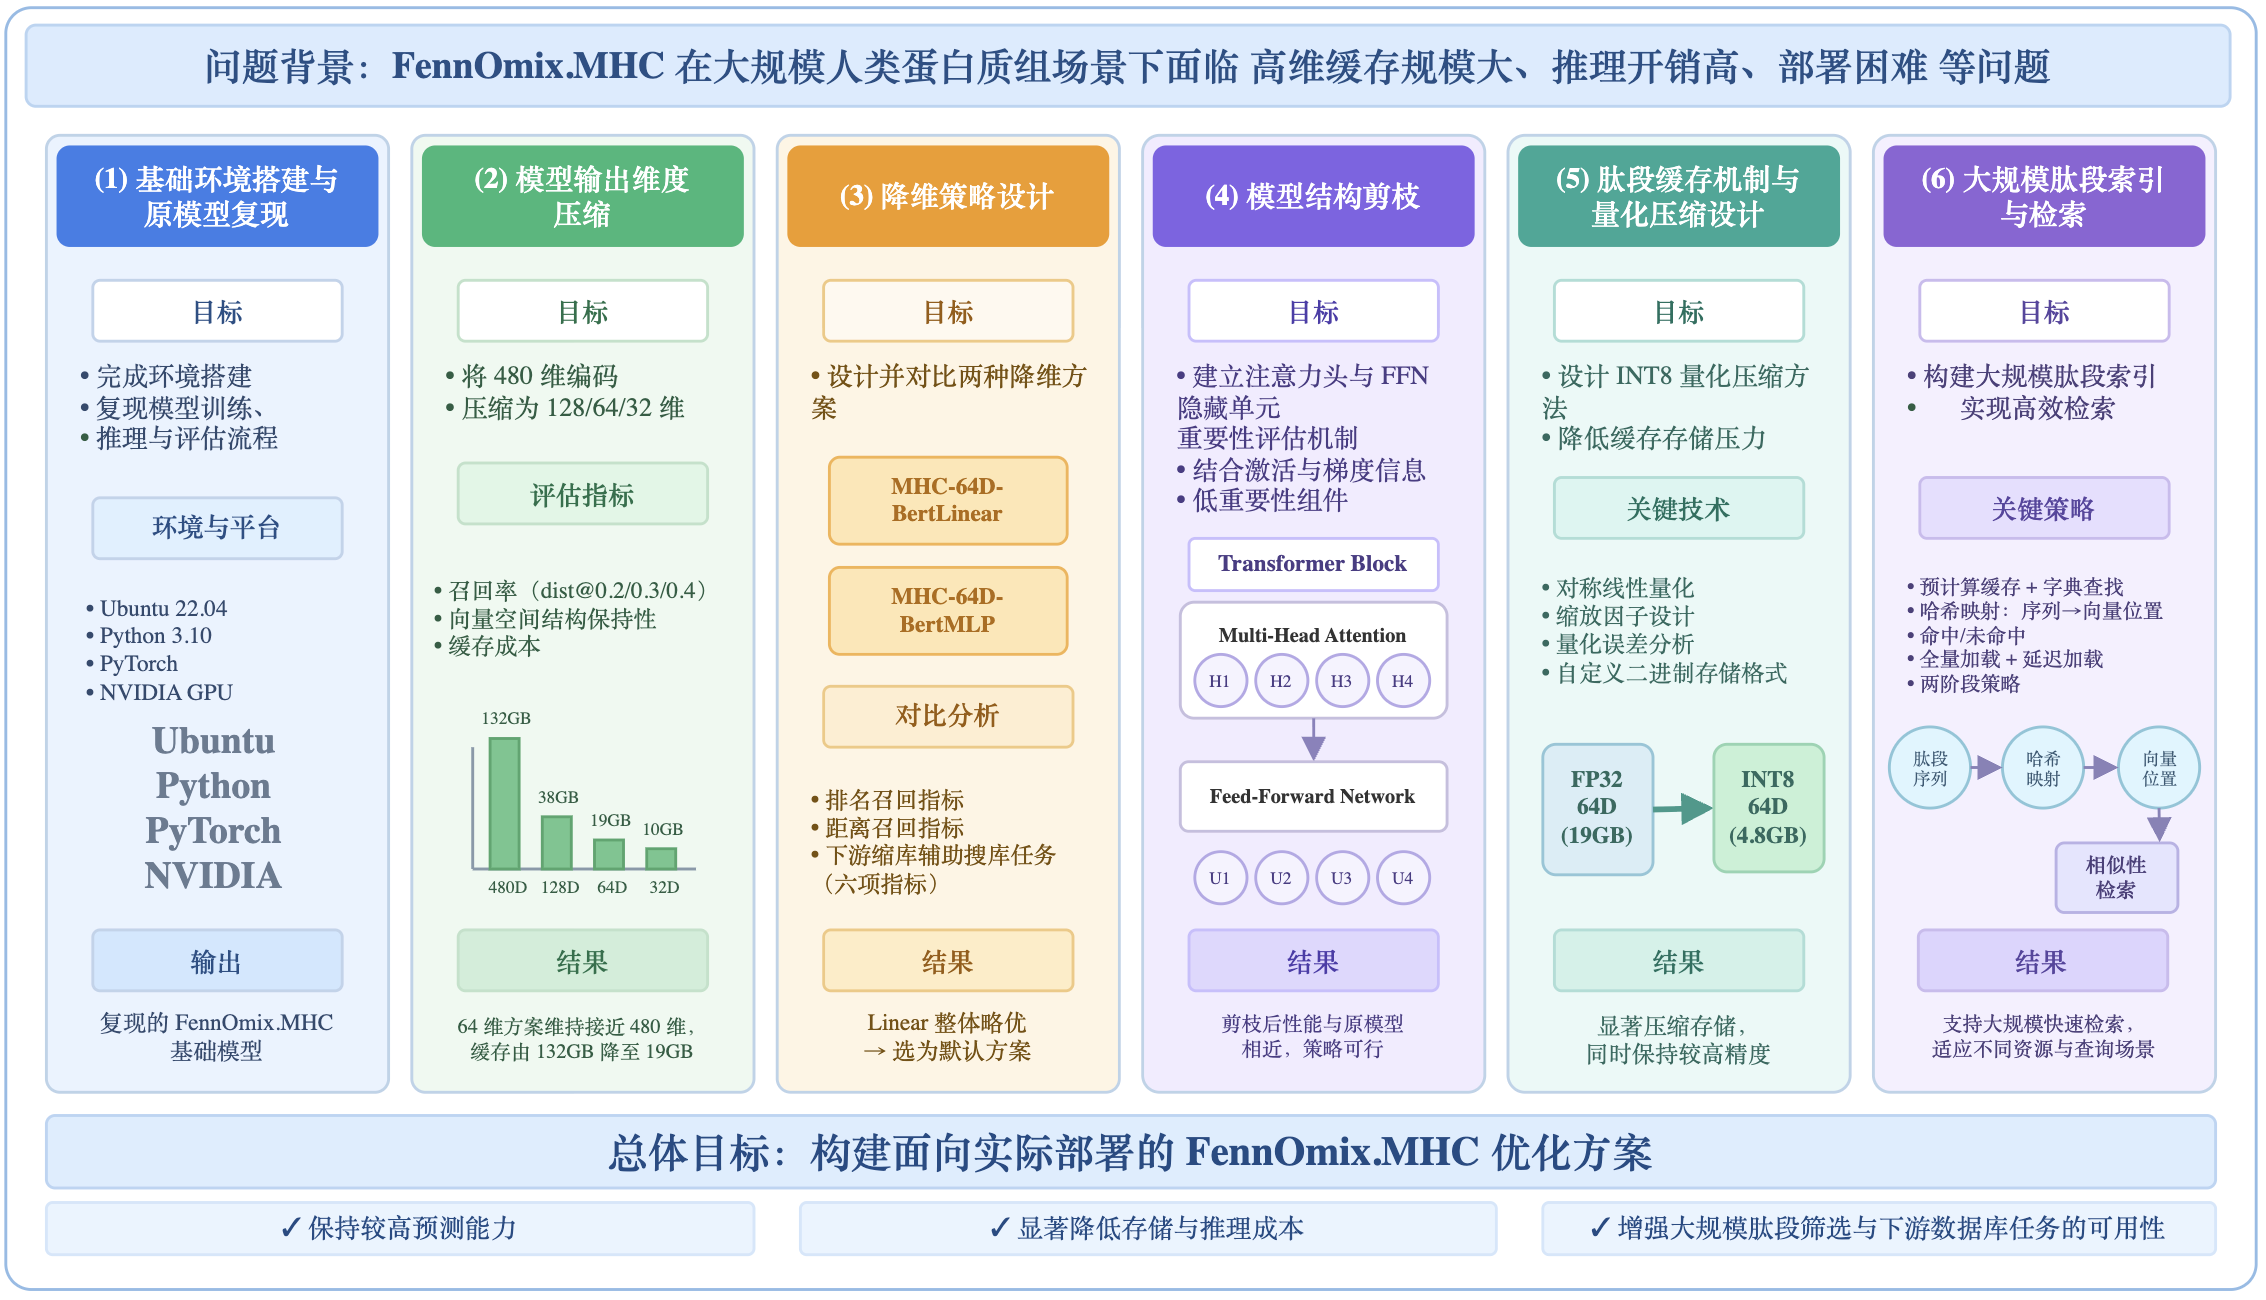
\includegraphics[width=1.0\textwidth]{figures/1.研究技术路线图.png}
\caption{模型优化与部署分析的研究技术路线图}
\label{fig:tech-route}
\end{figure}

% \section{本课题创新点}

% 结合已有研究基础和本文实际开展的工作，本课题的主要创新点概括如下。

% \begin{enumerate}[label=（\arabic*）, leftmargin=5em, itemsep=0pt, topsep=0pt]
%     \item 从实际部署需求出发，对 MHC-I 肽段结合预测模型进行轻量化研究。
%     \item 将表示压缩效果与下游缩库任务性能联动评价。
%     \item 在 FennOmix.MHC 的部署优化中引入结构冗余分析。
%     \item 构建模型优化与缓存、索引机制协同的部署流程。
% \end{enumerate}

\section{论文结构安排}

全文共分五章，具体安排如下。

第一章是绪论，介绍研究背景与意义，梳理国内外研究现状和现存问题，并明确本文的研究内容、创新点及整体结构。

第二章为理论基础与方法设计，将相关理论、模型轻量化策略和缓存索引机制整合论述。该章先交代MHC-I肽段结合预测任务、FennOmix.MHC基本框架、对比学习思想、评价指标以及缩库辅助数据库检索的基础，再围绕模型输出维度压缩、Linear与MLP降维方案、结构剪枝、INT8缓存压缩、自定义二进制格式、哈希索引和在线查询流程展开方法设计。

第三章是实验设计与结果分析，从实验环境、评价方法、不同输出维度比较、Linear与MLP模型对比、剪枝实验以及缓存压缩与索引机制效果等方面进行系统评估。

第四章为系统设计与部署分析，阐述轻量化模型、压缩缓存、索引检索与在线预测模块协同工作的整体流程，并分析系统在实际资源环境中的部署特征。

第五章是总结与展望，归纳全文工作，指出当前研究的局限，并对未来可进一步探索的方向进行展望。

\section{本章小结}

本章阐明了MHC-I肽段结合预测任务的背景与应用价值，分析了FennOmix.MHC在大规模候选肽段场景下所面临的高维缓存压力、存储开销和部署难题；继而回顾了相关研究进展与存在的短板，明确了本文的核心研究内容、创新点及章节安排。后续各章将在此基础上，依次推进模型轻量化、缓存压缩和系统部署优化等工作。